\documentclass[../main.tex]{subfiles}
\begin{document}
\newpage
\section{Инвариантность длины пути относительно допустимого преобразования переменной. Аддитивность длины пути.}
\emph{Путём} в \( \R ^n\) называется отображение \( \gamma \in C\left( \left[ a,b\right] \longrightarrow \R ^n\right),\quad a,b \in \R \).
Такая запись означает, что \( \gamma =\left( \gamma _1, \gamma _2, \dots, \gamma _n\right),\quad \forall \;i\quad \gamma _i \in C\left[ a,b\right]\). При этом \( \gamma _i\left( t\right)\) называется \(i\)-й координатой точки \( t\).

Лучше всего представлять это так, будто аргумент пути \( t\) - это время, а \( \gamma \left( t\right)\) - положение точки в этот момент времени. 

\( \gamma \) называется \emph{гладким}, если \( \forall \;i\quad \gamma _i \in C^1\left[ a,b\right]\). 

Если существует дробление \( \left\{ x_i\right\}_{i=1}^k:\quad \forall \;i=1\dots k\quad \gamma |_{\left[ x_{i-1}, x_i\right]}\) - гладкий путь, то 
\( \gamma \) называется \emph{кусочно-гладким}.

\InsertBoxR{0}{
    \begin{minipage}[t]{6cm} 
        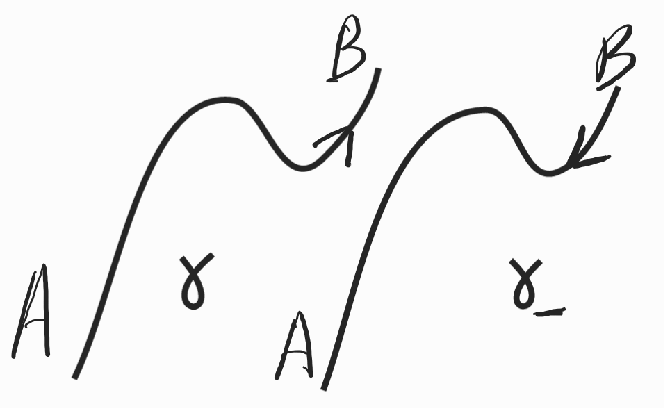
\includegraphics[width=\linewidth]{42_inverse.pdf} 
    \end{minipage}
}

\emph{Носителем пути} называется образ отрезка \( \left[ a,b\right]\) при отображении \( \gamma \).
\( \gamma \left( a\right)\) называется \emph{началом пути}, \( \gamma \left( b\right)\) называется \emph{концом пути}. 

Если \( \gamma :\left[ a,b\right] \longrightarrow \R ^n\) - путь, то отображение \( \gamma _-:\)\[\gamma _-(t)= \gamma \left( a+b-t\right),\quad t \in \left[ a,b\right]\]
называется \emph{противоположным путём} к \( \gamma \). 

~

Если \( \gamma \left( t_1\right)= \gamma \left( t_2\right) \implies t_1=t_2\), то \( \gamma \) называется \emph{простым (Жордановым) путём}. По факту это означает, что 
путь не имеет самопересечений. А если 
\begin{equation*}
    \gamma \left( t_1\right)= \gamma \left( t_2\right) \implies 
    \left[
    \begin{aligned}
        &\;t_1=t_2\\ 
        &\;\left\{ t_1,t_2\right\}=\left\{ a,b\right\}
    \end{aligned}
    \right.
\end{equation*}
то путь называется \emph{простым замкнутым}. То есть он имеет не больше одного самопересечения, которое является его началом и концом. 

~

Под \emph{кривой} часто понимают траекторию простого или простого замкнутого пути. Это первый подход к определению кривой.

Пути \( \gamma : \left[ a,b\right] \longrightarrow \R ^n\) и \( \tilde{ \gamma }: [ \tilde{a}, \tilde{b}] \longrightarrow \R ^n\) называются 
\emph{эквивалентными}, если существует строго возрастающая сюръективная функция \( \varphi :\left[ a,b\right] \longrightarrow [ \tilde{a}, \tilde{b}]\) такая что 
\[ \gamma = \tilde{ \gamma } \circ \varphi \]

\begin{note}
    Это действительно отношение эквивалентности.
    \begin{itemize}
        \item \emph{Рефлексивность:} можно просто взять \( \varphi \) как линейную функцию:
        \[ \varphi = \dfrac{ \tilde{b}-\tilde{a}}{ b-a}\left( x-a\right)+ \tilde{a}\]
        \item \emph{Симметричность:} так как от \( \varphi \) требуется, чтобы оно было строго монотонным, у него точно существует обратное отображение \( \tilde{ \varphi }\), которое тоже будет строго возрастающим. И тогда 
        \[ \tilde{ \gamma }= \gamma \circ \tilde{ \varphi }\]
        \item \emph{Транзитивность:}
        \begin{equation*}
            \begin{aligned}
                &\beta = \alpha \circ \varphi\\
                &\gamma = \beta \circ \chi
            \end{aligned}
            \implies \gamma = \alpha \circ \left( \varphi \circ \chi\right)
        \end{equation*}
        \( \varphi \circ \chi \) - искомое отображение. 
    \end{itemize}
\end{note}

\begin{example}

    ~

    \InsertBoxL{0}{
    \begin{minipage}[t]{7cm} 
        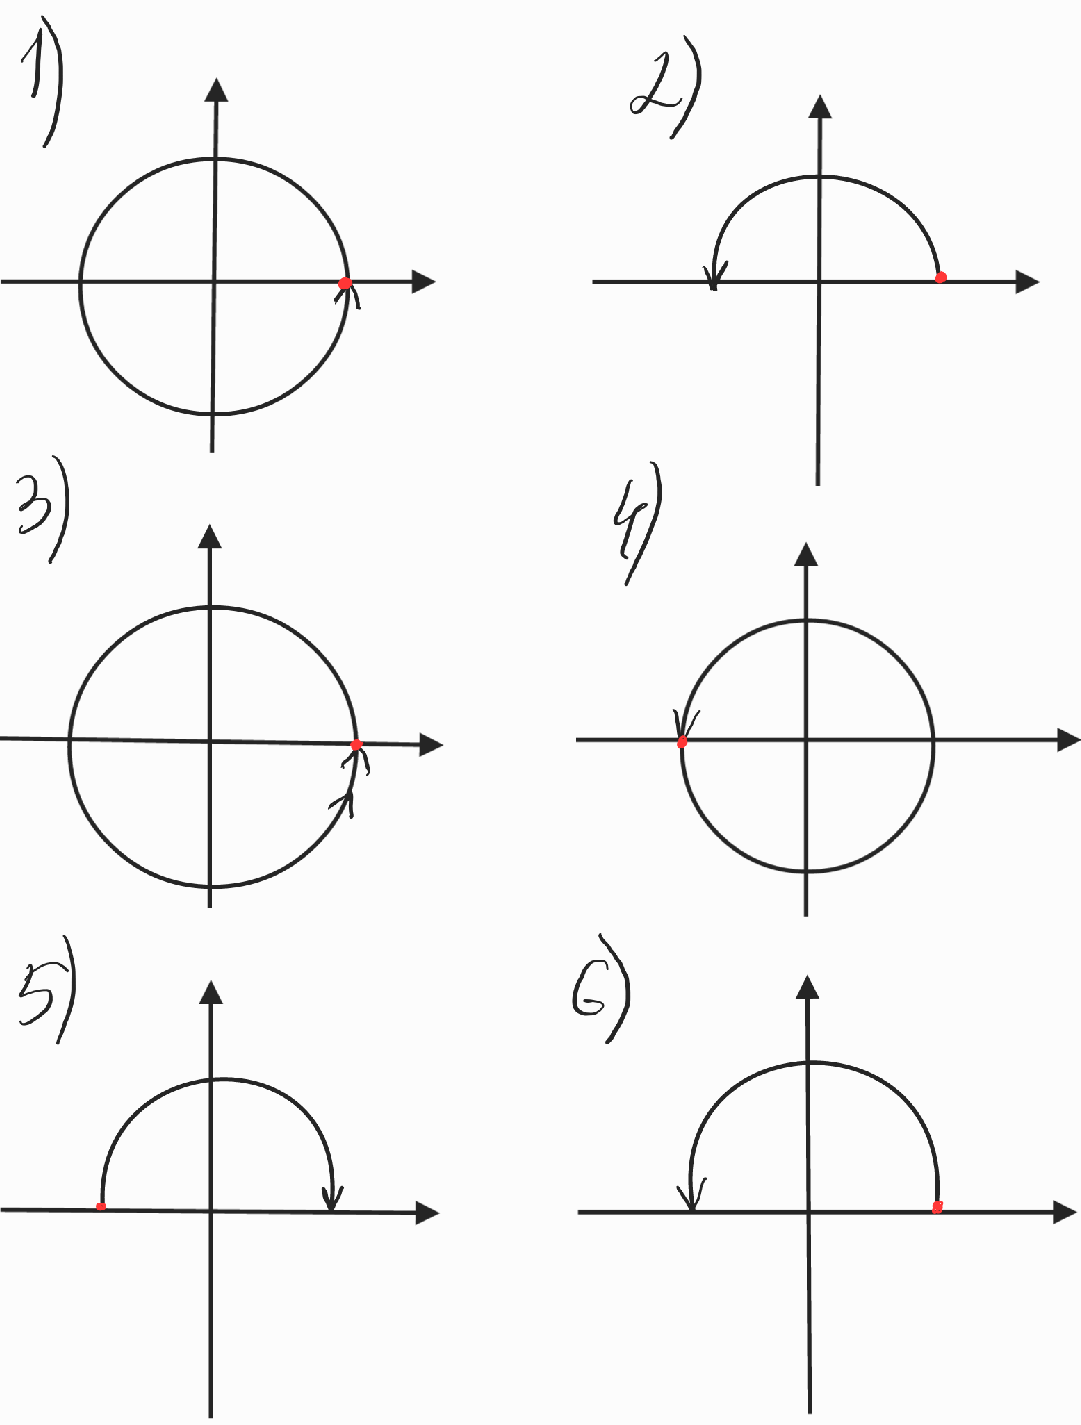
\includegraphics[width=0.9\linewidth]{42_circles.pdf} 
    \end{minipage}
    }
    \begin{equation*}
        \begin{aligned}
            &\gamma _1\left( t\right)= \left( \cos t, \sin t\right),\quad t \in \left[ 0, 2 \pi \right]\\
            &\gamma _2\left( t\right)=\left( \cos t, \sin t\right),\quad t \in \left[ 0, \pi \right]\\
            &\gamma _3\left( t\right)=\left( \cos t, \sin t\right),\quad t \in \left[ 0, 4 \pi \right]\\
            &\gamma _4\left( t\right)=\left( \cos t, \sin t\right),\quad t \in \left[ - \pi , \pi \right]\\
            &\gamma _5\left( t\right)=\left( t, \;\sqrt[]{1-t^2}\right),\quad t \in \left[ -1, 1\right]\\
            &\gamma _6\left( t\right)=\left( -t, \;\sqrt[]{1-t^2}\right),\quad t \in \left[ -1, 1\right]
        \end{aligned}
    \end{equation*}

    Разберём этот пример. Здесь все пути представляют из себя какие-то части окружностей. 
    Сначала нужно понять, что у эквивалентных путей обязательно должны совпадать начало и конец.

    \vspace{15mm}
    ~
     
    Так как отображение \( \varphi \) сюръективно и строго возрастает: 

    \begin{equation*}
        \begin{aligned}
            &\varphi \left( a\right)= \tilde{a}\\
            &\varphi \left( b\right)= \tilde{b}
        \end{aligned}
        \implies 
        \begin{aligned}
            &\gamma \left( a\right)= \tilde{ \gamma }\left( \tilde{a}\right)\\ 
            &\gamma\left( b\right)= \tilde{ \gamma }( \tilde{b}) 
        \end{aligned}
    \end{equation*}

    Таким образом, кандидатами в эквивалентные пути остаются только (1, 3) и (2, 6). Докажем, что если \( \gamma \) простой путь, то эквивалентный ему \( \tilde{ \gamma }\) тоже простой. 

    Пусть \( \gamma \) - простой путь, \( \tilde{ \gamma } \sim \gamma,\quad  \tilde{ \gamma }\left( t_1\right)= \tilde{ \gamma } \left( t_2\right),\quad t_1 \neq t_2\). Тогда 
    \[ \gamma \left( x_1\right)= \tilde{ \gamma }\left( \varphi \left( x_1\right)\right)= \tilde{ \gamma }\left( \varphi \left( x_2\right)\right)= \gamma \left( x_2\right)\]
    при \( \varphi \left( x_1\right) \neq \varphi \left( x_2\right)\). Но \( \varphi \) строго монотонна, а значит инъективна, поэтому \( x_1 \neq x_2\). Итого
    \[ \gamma \left( x_1\right)= \gamma \left( x_2\right),\quad x_1 \neq x_2\]
    чего быть не может по определению простого пути. Аналогично можно получить это утверждение для простого замкнутого пути. 

    Из этого следует, что 1 и 3 не могут быть эквивалентны. Остаются 2 и 6, они действительно эквивалентны, в этом можно убедиться, если в определении эквивалентных путей рассмотреть \( \varphi\left( x\right)=\dfrac{ \pi}{ 2}\left( x+1\right) \).
\end{example}

Если эквивалентность путей - это отношение эквивалентности, то оно должно разбивать множество путей на классы эквивалентности. 

\emph{Второй подход к определению кривой:} если \( \gamma :\left[ a,b\right] \longrightarrow \R \) - путь, то \( \left[ \gamma \right]\) (класс эквивалентности пути \( \gamma \)) называется \emph{кривой}, порождённой \( \gamma \). 
\[ \text{Г}=\left[ \gamma \right]\]
\\
Если Г - кривая, то для любого пути \( \gamma: \left[ \gamma \right]=\text{Г}\quad  \gamma \) называют \emph{параметризацией} Г.
\\
Кривая Г называется \emph{гладкой}, если существует гладкая параметризация Г.
\\
Кривая Г называется \emph{кусочно-гладкой}, если существует кусочно-гладкая параметризация Г.
\\
Кривая Г называется \emph{простой (Жордановой)}, если существует простая параметризация Г.
\\
Кривая Г называется \emph{замкнутой простой}, если существует замкнутая простая параметризация Г.

Если \( \gamma \), заданное на \( \left[ a,b\right]\) - путь и существует дробление \( X=\left( a=x_0, x_1, \dots,x_{n-1}, x_n=b\right)\) отрезка \( \left[ a,b\right]:\quad  \forall \; i=1 \dots n\quad \gamma |_{\left[ x_{i-1 },x_i\right]}\) - аффинная функция (то есть \( \forall \; k=1 \dots n\quad \gamma _k\left( t\right)=kt+b\)), тогда \( \gamma \) называется \emph{ломаной}. 

Пусть \( \gamma \) - ломаная, соединяющая точки \( \gamma \left( a\right)= \gamma \left( x_0\right), \gamma \left( x_1\right), \dots,  \gamma \left( x_{n-1}\right), \gamma \left( x_n\right)= \gamma \left( b\right)\)
\(  X=\left( x_0,x_1, \dots,x_n\right)\). Тогда длина ломаной \( \gamma \) равна 
\[ l \left(X, \gamma \right) = \sum\limits_{ i=1}^{ n} \left| \left| \gamma \left( x_i\right)- \gamma \left( x_{i-1}\right)\right|\right|\] 

Из определения следует, что длина ломаной неотрицательна. 

\InsertBoxR{0}{
    \begin{minipage}[t]{7cm} 
        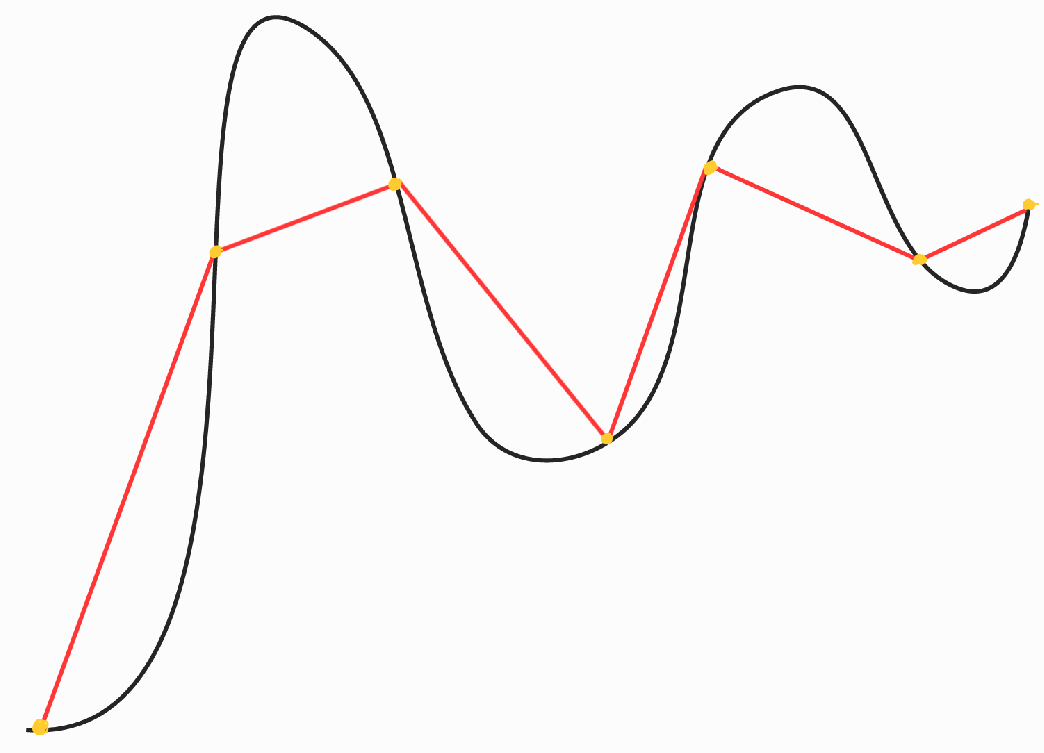
\includegraphics[width=0.9\linewidth]{42_path.pdf} 
    \end{minipage}
}

Длина пути определяется как супремум длин ломаных, которыми можно приближать этот путь. Конечно, она тоже неотрицательна. Более формально: если \( \gamma \) - путь, то длина пути \( \gamma \) равна 
\[ s\left(\gamma \right)= \sup\limits_{ X\text{-дробление }\left[ a,b\right]} l \left( X, \gamma \right)\]

Супремум существует всегда, но не обязательно является конечным, то есть может быть равен \( + \infty \). Если \( s\left( \gamma \right)<+ \infty \), то \( \gamma \) называется \emph{спрямляемым}.  

\begin{thm}[Равенство длин эквивалентных путей]
    \[ \gamma \sim \tilde{ \gamma } \implies s\left( \gamma \right)=s\left( \tilde{ \gamma }\right)\]
\end{thm}

\begin{proof}
    
    ~
    
    Сначала стоит отметить такой факт: если \( M\) - множество, \( \forall \; x \in M\quad x \leq a\), тогда \( \sup\limits_{ } M \leq a\). Этот факт напрямую следует из определения супремума как наименьшей мажоранты. Этот факт часто будет использован
    при доказательстве утверждений, связанных с путями, в том числе и в этом доказательстве. 
    
    План такой: мы докажем, что \( s\left( \gamma \right) \leq s\left( \tilde{ \gamma }\right)\). 
    Для этого докажем, что \( \forall \; X\) - дробления промежутка \( \left[ a,b\right]\quad l \left( X, \gamma \right) \leq s\left( \tilde{ \gamma }\right)\), затем перейдём к супремуму. Потом мы проведём точно такие же рассуждения, доказывая что \( s\left( \tilde{ \gamma }\right) \leq s\left( \gamma \right)\), и получим \( s\left( \gamma \right)=s\left( \tilde{ \gamma }\right)\).

    Пусть \( \gamma \) действует на \( \left[ a,b\right]\), \( \tilde{ \gamma }\) действует на \( [ \tilde{ a}, \tilde{ b}]\). По определению эквивалентных путей 
    \[ \exists \; \varphi : \left[ a,b\right] \longrightarrow [ \tilde{ a}, \tilde{ b}],\quad \gamma = \tilde{ \gamma }\circ \varphi ,\quad \varphi \text{ - строго монотонна}\]

    Обозначим \( \tilde{ X}=( \tilde{ x}_0, \tilde{ x}_1, \dots, \tilde{ x}_n)=( \varphi \left( x_0\right), \varphi \left( x_1\right), \dots, \varphi \left( x_n\right))\).
    \begin{equation*}
        \begin{aligned}
            &l \left( X, \gamma \right)= \sum\limits_{ i=1}^{ n} \left| \left| \gamma \left( x_i\right)- \gamma \left( x_{i-1}\right)\right|\right|= \sum\limits_{ i=1}^{ n} \left| \left| \tilde\gamma \left( \varphi \left( x_i\right)\right)- \tilde{ \gamma }\left( \varphi \left( x_{i-1}\right)\right)\right|\right|=\\ 
            &= \sum\limits_{ i=1}^{ n} \left| \left| \tilde{ \gamma }\left( \tilde{ x}_i\right)- \tilde{ \gamma }\left( \tilde{ x}_{i-1}\right)\right|\right|=l ( \tilde{ X}, \tilde{ \gamma }) \leq \sup\limits_{ \tilde{ X}\text{-дробление}[ \tilde{ a}, \tilde{ b}]} l ( \tilde{ X}, \tilde{ \gamma })=s\left( \tilde{ \gamma }\right)
        \end{aligned}
    \end{equation*}

    Таким образом, \( l \left( X, \gamma \right) \leq s\left( \tilde{ \gamma }\right) \implies s\left( \gamma \right)= \sup\limits_{ } l \left( X, \gamma \right) \leq s\left( \tilde{ \gamma }\right)\) 

    Так как условие симметрично относительно \( \gamma \) и \( \tilde{ \gamma }\), мы можем провести аналогичные рассуждения, поменяв местами \( \gamma \) и \( \tilde{ \gamma }\) и прийти к выводу \( s\left( \tilde\gamma \right) \leq s\left( \gamma \right)\)

    \begin{equation*}
        \begin{aligned}
            s\left( \gamma \right) \leq s\left( \tilde{ \gamma }\right)\\ 
            s\left( \tilde{ \gamma }\right) \leq s\left( \gamma \right)
        \end{aligned}
        \implies 
        s\left( \gamma \right)=s\left( \tilde{ \gamma }\right)
    \end{equation*}
\end{proof}

Так как длина всей путей в одном классе эквивалентности одна и та же, говорят о \emph{длине кривой}. Длина кривой - длина любой её параметризации.

\begin{thm}[Равенство длин противоположных путей]
    \[ \tilde{ \gamma }\text{ - противоположный путь к } \gamma \implies s( \tilde{ \gamma })=s\left( \gamma \right)\]
\end{thm}
\begin{proof}
    Доказательство почти аналогично предыдущей теореме. 

    Пусть \( \gamma , \tilde{ \gamma }\) действуют на \( \left[ a,b\right],\quad \forall \; t \in \left[ a,b\right]\quad \tilde{ \gamma }\left( t\right)= \gamma \left( a+b-t\right),\)
    \( X=(a+b-x_1,a+b-x_2, \dots,a+b-x_n),\quad \tilde{ X}=(x_1, x_2, \dots, x_n)\)

    \begin{equation*}
        \begin{aligned}
            l \left( X, \gamma \right)&= \sum\limits_{ i=1}^{ n} \left| \left| \gamma \left( a+b-x_i\right)- \gamma \left( a+b-x_{i-1}\right)\right|\right|= \sum\limits_{ i=1}^{ n} \left| \left| \tilde{ \gamma }\left( x_i\right)- \tilde{ \gamma }\left( x_{i-1}\right)\right|\right|=\\
            &=l( \tilde{ X}, \tilde{ \gamma }) \leq \sup\limits_{ } l( \tilde{ X}, \tilde{ \gamma })=s( \tilde{ \gamma } )
        \end{aligned}
    \end{equation*}
    
    Переходя к супремуму, получим \( s\left( \gamma \right) \leq s\left( \tilde{ \gamma }\right)\). Но если \( \tilde{ \gamma }\) - противоположный к \( \gamma \), то \( \gamma \) - противоположный к \( \tilde{ \gamma }\). Тогда проведя аналогичные рассуждения, поменяв местами \( \gamma \) и \( \tilde{ \gamma }\), получим \( s( \tilde{ \gamma }) \leq s\left( \gamma \right)\)

    \begin{equation*}
        \begin{aligned}
            s\left( \gamma \right) \leq s\left( \tilde{ \gamma }\right)\\ 
            s\left( \tilde{ \gamma }\right) \leq s\left( \gamma \right)
        \end{aligned}
        \implies 
        s\left( \gamma \right)=s\left( \tilde{ \gamma }\right)
    \end{equation*}
\end{proof}

\begin{note}
    \hypertarget{note:add_point_in_x}{Когда мы приближаем длину пути длиной ломаной, при добавлении точки в дробление длина ломаной увеличивается. }

    \begin{equation*}
        \begin{aligned}
            &X=\left( x_0, x_1, \dots, x_n\right)\\ 
            &\tilde{ X}=(\tilde{ x}_0, \tilde{ x}_1, \dots, \tilde{ x}_{k-1},c, \tilde{ x}_k, \dots, \tilde{ x}_n)
        \end{aligned}
        \text{- дробления } \left[ a,b\right]
    \end{equation*}
    Тогда 
    \[ l \left( X, \gamma \right) \leq l( \tilde{ X}, \gamma ) \]
\end{note}
\begin{proof}
    \(l\left( X, \gamma \right)= \sum\limits_{ i=1}^{ n} \left| \left| \gamma \left( x_i\right)- \gamma \left( x_{i-1}\right)\right|\right|\)\\
    \begin{equation*}
        \begin{aligned}
            &l( \tilde{ X}, \gamma)= \sum\limits_{i=1, i \neq k}^{n} \left| \left| \gamma \left( x_i\right)- \gamma \left( x_{i-1}\right)\right|\right|+ \underbrace{\left| \left| \gamma \left( c\right)- \gamma \left( x_{k-1}\right)\right|\right|+\left| \left| \gamma \left( x_k\right)- \gamma \left( c\right)\right|\right|}_{ \geq \left| \left| \gamma \left( x_k\right)- \gamma \left( x_{k-1}\right)\right|\right| \text{ по нер-ву треугольника}} \geq\\
            &\geq \sum\limits_{ i=1}^{ n} \left| \left| \gamma \left( x_i\right)- \gamma \left( x_{i-1}\right)\right|\right|=l \left( X, \gamma \right)
        \end{aligned}
    \end{equation*}
\end{proof}

\begin{thm}[\hypertarget{thm:path_add}{Аддитивность длины пути}]
    \( \Let \; \gamma :\left[ a,b\right] \longrightarrow \R ^n\) - путь, 
    \[ c \in \left( a,b\right),\quad \gamma _-= \gamma |_{\left[ a,c\right]},\quad \gamma _+= \gamma |_{\left[ c,b\right]}\]
    Тогда 
    \[ s\left( \gamma \right)=s\left( \gamma _-\right)+s\left( \gamma _+\right)\]
\end{thm}
\begin{proof}
    Доказывать будем 2 неравенства: \( s\left( \gamma _-\right)+s\left( \gamma _+\right) \leq s\left( \gamma \right)\) и \( s\left( \gamma _-\right)+s\left( \gamma _+\right) \geq s\left( \gamma \right)\),
    откуда получим требуемое. 

    Рассмотрим два произвольных дробления отрезков \(\left[ a,c\right]\) и \( \left[ c,b\right]\).

    \( X_-=\left( x_0, x_1, \dots, x_k, c\right)\text{ - дробление } \left[ a,c\right],\quad X_+=\left( c, x_{k+1}, \dots, x_n\right)\text{ - дробление } \left[ c,b\right]\)

    \( \Let \; X =\left( x_0, x_1, \dots, x_k, c, x_{k+1}, \dots, x_n\right)\text{ - дробление}  \left[ a,b\right]\)

    \begin{equation}\label{lab:eq:path_addition}
        \begin{aligned}
            &l \left( X_-, \gamma _-\right)+l \left( X_+, \gamma _+\right)=\\
            &= \sum\limits_{ i=1}^{ k} \left| \left| \gamma _-\left( x_i\right)- \gamma _-\left( x_{i-1}\right)\right|\right|+ \left| \left| \gamma _-\left( c\right)- \gamma _-\left( x_k\right)\right|\right|+\\
            &+\left| \left| \gamma _+\left( x_{k+1}\right)- \gamma _+\left( c\right)\right|\right|+\sum\limits_{ i=k+1}^{ n} \left| \left| \gamma_+\left( x_i\right)-\gamma _+\left( x_{i-1}\right) \right|\right|=\\
            &= \sum\limits_{ i=1}^{ k} \left| \left| \gamma\left( x_i\right)- \gamma \left( x_{i-1}\right)\right|\right|+ \left| \left| \gamma \left( c\right)- \gamma \left( x_k\right)\right|\right|+\left| \left| \gamma \left( x_{k+1}\right)- \gamma \left( c\right)\right|\right|+\sum\limits_{ i=k+1}^{ n} \left| \left| \gamma\left( x_i\right)-\gamma \left( x_{i-1}\right) \right|\right|=\\
            &= \sum\limits_{ i=1}^{ n} \left| \left| \gamma\left( x_i\right)- \gamma \left( x_{i-1}\right)\right|\right|+ \left| \left| \gamma \left( c\right)- \gamma \left( x_k\right)\right|\right|+\left| \left| \gamma \left( x_{k+1}\right)- \gamma \left( c\right)\right|\right|=l(X, \gamma )
        \end{aligned}
    \end{equation}

    Получили равенство \(l \left( X_-, \gamma _-\right)+l\left( X_+, \gamma _+\right)=l\left( X, \gamma \right)\).

    Перейдём в нём к супремуму в правой части, это можно сделать всегда: 
    \[ l \left( X_-, \gamma _-\right)+l \left( X_+, \gamma _+\right) \leq s\left( \gamma \right)\]

    Теперь по очереди к перейдём к двум супремумам в левой части. Это можно сделать, так как неравенство выше верно для произвольных \( X_-, X_+\) 
    \[ s\left( \gamma _-\right)+s\left( \gamma _+\right) \leq s\left( \gamma \right)\]

    Теперь хотим доказать обратное неравенство. Пусть \( X\) - произвольное дробление \( \left[ a,b\right]\).

    Если \( c \in X \implies X=\left( x_0,x_1, \dots,x_{k-1},c,x_k, \dots,x_n\right)\). Пройдя в цепочке равенств \ref{lab:eq:path_addition} снизу вверх, получим:
    \[ l \left( X, \gamma \right)=l\left( \left( x_0, x_1, \dots,x_{k-1},c\right), \gamma _-\right)+l \left( \left( c,x_k, \dots,x_n\right), \gamma _+\right)\]

    Перейдём к супремуму в правой части, это можно сделать всегда:
    \[ l \left( X, \gamma \right) \leq s\left( \gamma _-\right)+s\left( \gamma _+\right)\]

    Если \( c \notin X \implies \exists \; k \in \left\{ 1, \dots,n\right\}:\;c \in \left[ x_{k-1}, x_k\right]\). Добавим точку \( c\) в дробление 
    \( X\), получим дробление \( \tilde{ X}=\left( x_0,x_1, \dots,x_{k-1}, c, x_k, \dots, x_n\right)\). По \hyperlink{note:add_point_in_X}{замечанию} мы знаем, что
    длина ломаной при добавлении точки не уменьшается, а \( \tilde{ X}\) уже содержит точку \( c\) и попадает под случай выше:
    \[ l \left( X, \gamma \right) \leq l ( \tilde{ X}, \gamma ) \leq s\left( \gamma _-\right)+s\left( \gamma _+\right)\]

    Поэтому для любого дробления \( X\) верно \( l \left( X, \gamma \right) \leq s\left( \gamma _-\right)+s\left( \gamma _+\right)\), значит мы можем перейти к супремуму в левой части неравенства:
    \[ s\left( \gamma \right) \leq s\left( \gamma _-\right)+s\left( \gamma _+\right)\]
    \begin{equation*}
        \begin{aligned}
            &s\left( \gamma \right) \leq s\left( \gamma _-\right)+s\left( \gamma _+\right)\\ 
            &s\left( \gamma _-\right)+s\left( \gamma _+\right) \leq s\left( \gamma \right)
        \end{aligned}
        \implies 
        s\left( \gamma \right)=s\left( \gamma _-\right)+s\left( \gamma _+\right)
    \end{equation*}
\end{proof}
\end{document}